\documentclass{article}

\usepackage{graphicx}
\usepackage{tikz}
\usepackage{tikzsymbols}
\usetikzlibrary{calc,patterns,shapes.geometric}
\pagestyle{empty}
\usepackage[margin=0pt]{geometry}
\geometry{papersize={14in,12in}}

\def\centerarc[#1](#2)(#3:#4:#5){\draw[#1] ($(#2)+({#5*cos(#3)},{#5*sin(#3)})$) arc (#3:#4:#5);}

\begin{document}
	\begin{figure}
		\centering
		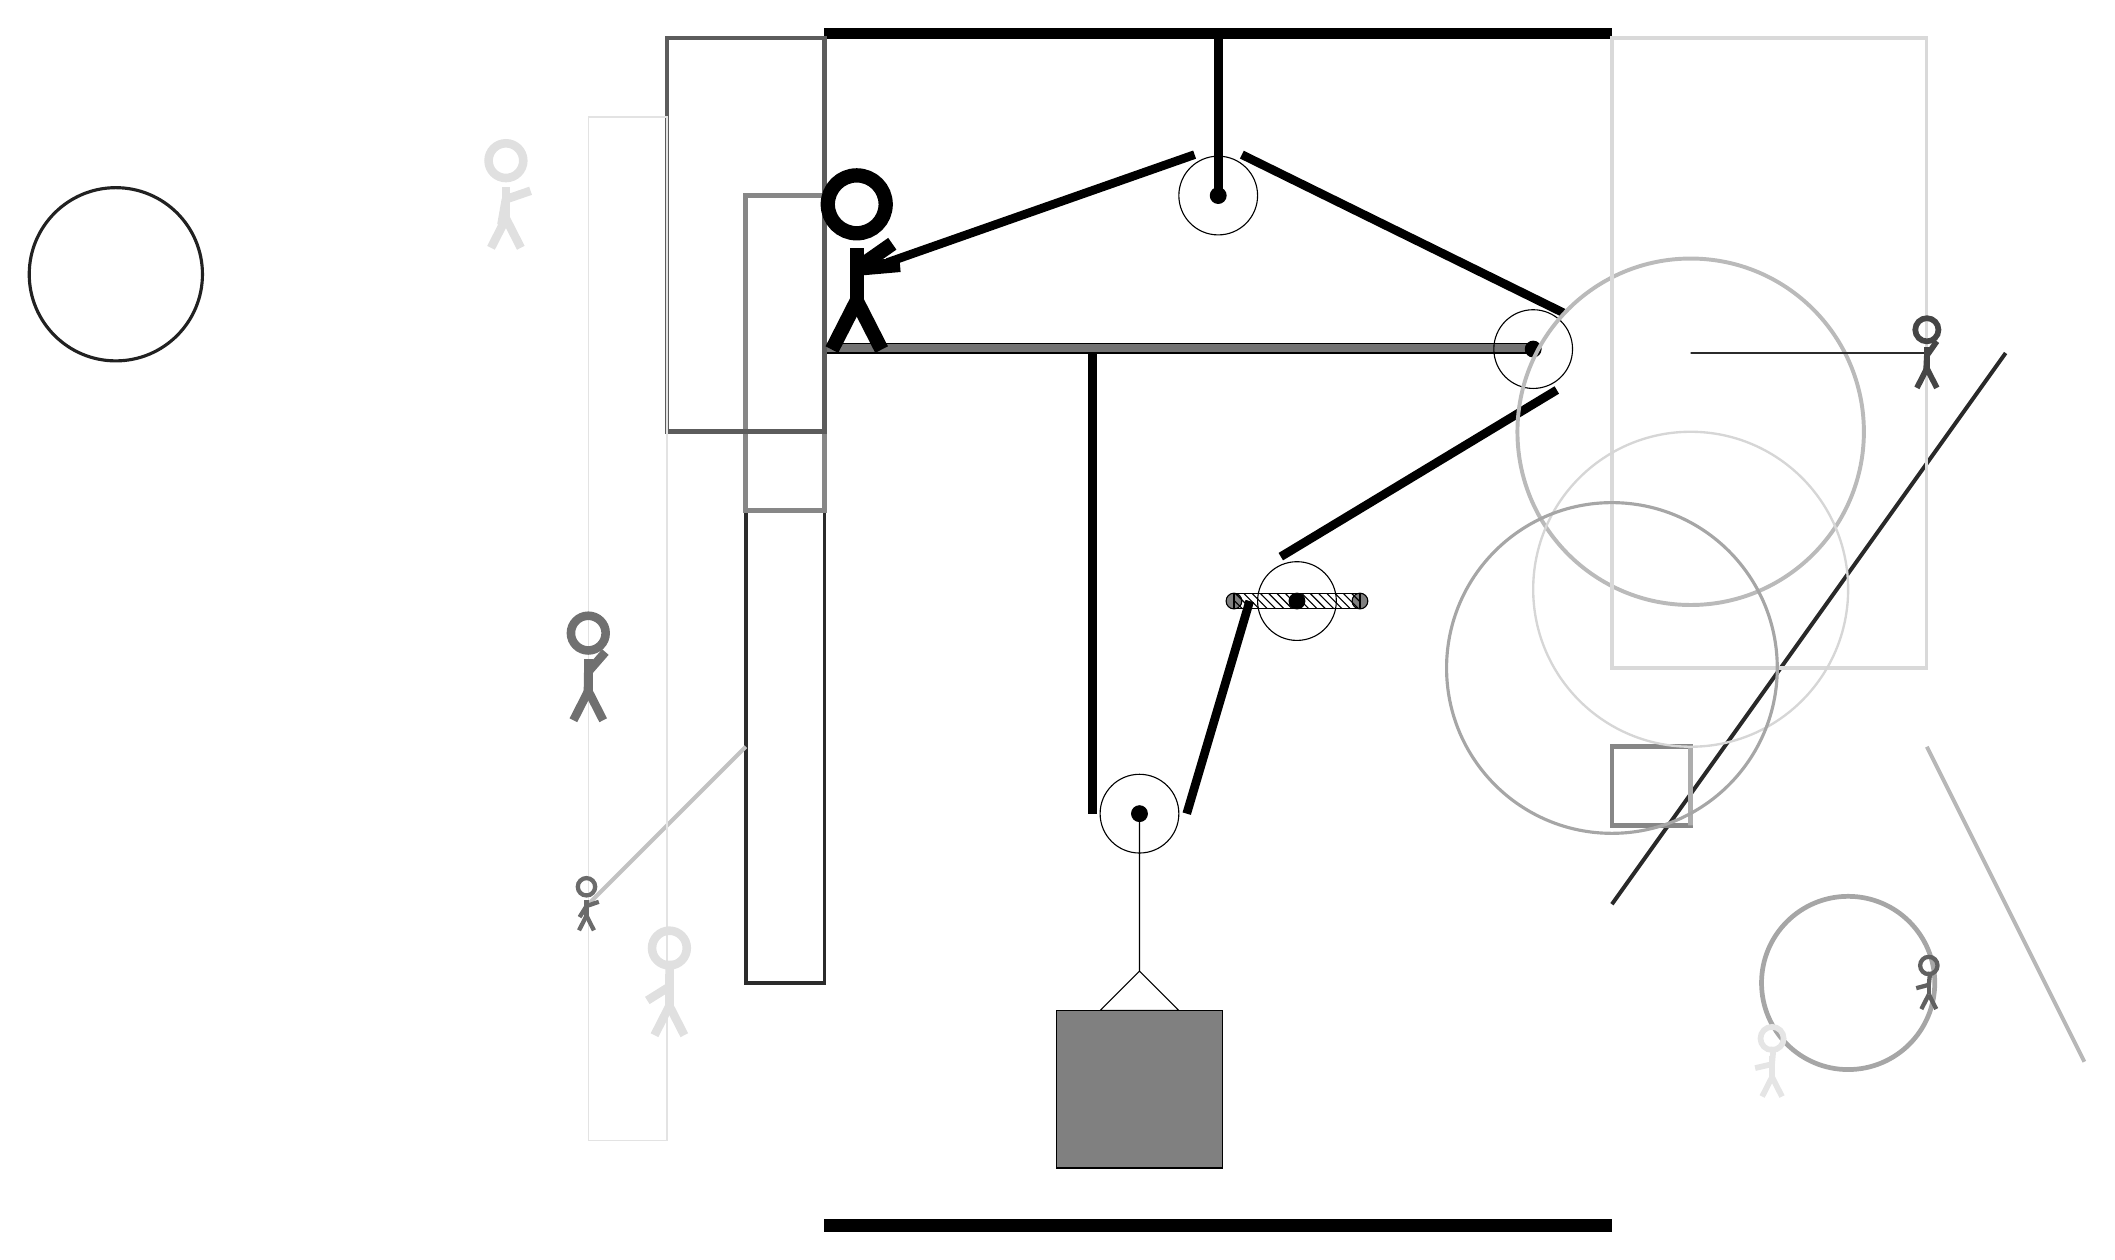
\begin{tikzpicture}
			%%%%% START %%%%%
			
			\draw[fill=black] (-2, 13) rectangle (8, 13.125);
			
			\draw[fill=black!55] (-2, 9) rectangle (7, 9.125);
			
			\draw (2, 3.15) circle (0.5);
			\draw[fill=black] (2, 3.15) circle (0.1);
			
			\draw (7, 9.05) circle (0.5);
			\draw[fill=black] (7, 9.05) circle (0.1);
			
			\draw[fill=white](4, 5.85) circle (0.5);
			\draw[fill=black] (4, 5.85) circle (0.1);
			\draw[fill=black!50] (3.2, 5.85) circle (0.1);
			\draw[fill=black!50] (4.8, 5.85) circle (0.1);
			\draw[pattern=north west lines, pattern color=black] (3.2, 5.95) rectangle (4.8, 5.75);
			
			\draw (3, 11) circle (0.5);
			\draw[fill=black] (3, 11) circle (0.1);
			\draw[line width=1.1mm] (3, 11) -- (3, 13);
			
			\draw (2, 3.15) -- (2, 1.15) -- (1.5, 0.65) -- (2.5, 0.65) -- (2, 1.15);
			\draw[fill=black!50] (0.95, 0.65) rectangle (3.05, -1.35);
			
			\draw[line width=1.1mm] (1.4, 9) -- (1.4, 3.15);
			\centerarc[line width=1.1mm](2, 3.15)(180:360:0.6);
			\draw[line width=1.1mm](2.6, 3.15) -- (3.4, 5.85);
			\centerarc[line width=1.1mm](4, 5.85)(110:180:0.6);
			\draw[line width=1.1mm](3.7948, 6.4138) -- (7.3, 8.5304);
			\centerarc[line width=1.1mm](7, 9.05)(-60:50:0.6);
			\draw[line width=1.1mm](7.3857, 9.5096) -- (3.3, 11.5196);
			\centerarc[line width=1.1mm](3, 11)(60:120:0.6);
			\draw[line width=1.1mm](2.7, 11.5196) -- (-1.2, 10.15);
			
			\draw [line width=0.6mm, color=black!35](11, 1) circle (1.1);
			
			\node[line width=0.5mm, color=black!62] at (12, 1) {\Strichmaxerl[3][15][84]};
			\draw [line width=0.4mm, color=black!87](-11, 10) circle (1.1);
			\draw[line width=0.5mm, color=black!83] (-2, 11) rectangle (-3, 1);
			
			\draw[line width=0.6mm, color=black!47] (-3, 7) rectangle (-2, 11);
			
			\draw[line width=0.5mm, color=black!84](13, 9) -- (8, 2);
			
			\draw [line width=0.5mm, color=black!27](9, 8) circle (2.2);
			\draw[line width=0.5mm, color=black!28](12, 4) -- (14, 0);
			\draw[line width=0.4mm, color=black!15] (8, 13) rectangle (12, 5);
			\draw[line width=0.6mm, color=black!47] (8, 4) rectangle (9, 3);
			\draw[line width=0.6mm, color=black!32] (9, 3) rectangle (9, 4);
			\draw[line width=0.5mm, color=black!24](-5, 2) -- (-3, 4);
			\draw[line width=0.2mm, color=black!83] (9, 9) rectangle (12, 9);
			
			\draw[line width=0.6mm, color=black!64] (-4, 13) rectangle (-2, 8);
			\draw [line width=0.3mm, color=black!16](9, 6) circle (2.0);
			\draw [line width=0.4mm, color=black!35](8, 5) circle (2.1);
			
			\draw[line width=0.2mm, color=black!11] (-4, 12) rectangle (-5, -1);
			\node[line width=0.4mm, color=black!73] at (12, 9) {\Strichmaxerl[4][87][55]};
			\node[line width=0.7mm, color=black!10] at (10, 0) {\Strichmaxerl[4][13][85]};
			\node[line width=0.3mm, color=black!56] at (-5, 5) {\Strichmaxerl[6][89][49]};
			\node[line width=0.5mm, color=black!12] at (-4, 1) {\Strichmaxerl[6][32][89]};
			
			\node[line width=0.4mm, color=black!12] at (-6, 11) {\Strichmaxerl[6][80][19]};
			
			\node[line width=0.7mm, color=black!58] at (-5, 2) {\Strichmaxerl[3][58][19]};
			
			\node at (-1.5, 10.15) {\Strichmaxerl[10][-175][35]};
			
			\draw[fill=black] (-2, -2) rectangle (8, -2.15);
			
			%%%%% END %%%%%
		\end{tikzpicture}
	\end{figure}	
\end{document}